\documentclass[journal,12pt,twocolumn]{IEEEtran}
%
\usepackage{setspace}
\usepackage{gensymb}
\usepackage{xcolor}
\usepackage{caption}
\usepackage{circuitikz}
%\usepackage{subcaption}
%\doublespacing
\singlespacing
\usepackage{float}
%\usepackage{graphicx}
%\usepackage{amssymb}
%\usepackage{relsize}
\usepackage[cmex10]{amsmath}
\usepackage{mathtools}
%\usepackage{amsthm}
%\interdisplaylinepenalty=2500
%\savesymbol{iint}
%\usepackage{txfonts}
%\restoresymbol{TXF}{iint}
%\usepackage{wasysym}
\usepackage{hyperref}
\usepackage{amsthm}
\usepackage{mathrsfs}
\usepackage{txfonts}
\usepackage{stfloats}
\usepackage{cite}
\usepackage{cases}
\usepackage{subfig}
%\usepackage{xtab}
\usepackage{longtable}
\usepackage{multirow}
%\usepackage{algorithm}
%\usepackage{algpseudocode}
%\usepackage{enumerate}
\usepackage{enumitem}
\usepackage{mathtools}
%\usepackage{iithtlc}
%\usepackage[framemethod=tikz]{mdframed}
\usepackage{listings}
\let\vec\mathbf


%\usepackage{stmaryrd}


%\usepackage{wasysym}
%\newcounter{MYtempeqncnt}
\DeclareMathOperator*{\Res}{Res}
%\renewcommand{\baselinestretch}{2}
\renewcommand\thesection{\arabic{section}}
\renewcommand\thesubsection{\thesection.\arabic{subsection}}
\renewcommand\thesubsubsection{\thesubsection.\arabic{subsubsection}}

\renewcommand\thesectiondis{\arabic{section}}
\renewcommand\thesubsectiondis{\thesectiondis.\arabic{subsection}}
\renewcommand\thesubsubsectiondis{\thesubsectiondis.\arabic{subsubsection}}

%\renewcommand{\labelenumi}{\textbf{\theenumi}}
%\renewcommand{\theenumi}{P.\arabic{enumi}}

% correct bad hyphenation here
\hyphenation{op-tical net-works semi-conduc-tor}

\lstset{
language=Python,
frame=single, 
breaklines=true,
columns=fullflexible
}



\begin{document}
%

\theoremstyle{definition}
\newtheorem{theorem}{Theorem}[section]
\newtheorem{problem}{Problem}
\newtheorem{proposition}{Proposition}[section]
\newtheorem{lemma}{Lemma}[section]
\newtheorem{corollary}[theorem]{Corollary}
\newtheorem{example}{Example}[section]
\newtheorem{definition}{Definition}[section]
%\newtheorem{algorithm}{Algorithm}[section]
%\newtheorem{cor}{Corollary}
\newcommand{\BEQA}{\begin{eqnarray}}
\newcommand{\EEQA}{\end{eqnarray}}
\newcommand{\define}{\stackrel{\triangle}{=}}
\newcommand{\myvec}[1]{\ensuremath{\begin{pmatrix}#1\end{pmatrix}}}
\newcommand{\mydet}[1]{\ensuremath{\begin{vmatrix}#1\end{vmatrix}}}

\bibliographystyle{IEEEtran}
%\bibliographystyle{ieeetr}

\providecommand{\nCr}[2]{\,^{#1}C_{#2}} % nCr
\providecommand{\nPr}[2]{\,^{#1}P_{#2}} % nPr
\providecommand{\mbf}{\mathbf}
\providecommand{\pr}[1]{\ensuremath{\Pr\left(#1\right)}}
\providecommand{\qfunc}[1]{\ensuremath{Q\left(#1\right)}}
\providecommand{\sbrak}[1]{\ensuremath{{}\left[#1\right]}}
\providecommand{\lsbrak}[1]{\ensuremath{{}\left[#1\right.}}
\providecommand{\rsbrak}[1]{\ensuremath{{}\left.#1\right]}}
\providecommand{\brak}[1]{\ensuremath{\left(#1\right)}}
\providecommand{\lbrak}[1]{\ensuremath{\left(#1\right.}}
\providecommand{\rbrak}[1]{\ensuremath{\left.#1\right)}}
\providecommand{\cbrak}[1]{\ensuremath{\left\{#1\right\}}}
\providecommand{\lcbrak}[1]{\ensuremath{\left\{#1\right.}}
\providecommand{\rcbrak}[1]{\ensuremath{\left.#1\right\}}}
\theoremstyle{remark}
\newtheorem{rem}{Remark}
\newcommand{\sgn}{\mathop{\mathrm{sgn}}}
\providecommand{\abs}[1]{\left\vert#1\right\vert}
\providecommand{\res}[1]{\Res\displaylimits_{#1}} 
\providecommand{\norm}[1]{\lVert#1\rVert}
\providecommand{\mtx}[1]{\mathbf{#1}}
\providecommand{\mean}[1]{E\left[ #1 \right]}
\providecommand{\fourier}{\overset{\mathcal{F}}{ \rightleftharpoons}}
\providecommand{\ztrans}{\overset{\mathcal{Z}}{ \rightleftharpoons}}

%\providecommand{\hilbert}{\overset{\mathcal{H}}{ \rightleftharpoons}}
\providecommand{\system}{\overset{\mathcal{H}}{ \longleftrightarrow}}
	%\newcommand{\solution}[2]{\textbf{Solution:}{#1}}
\newcommand{\solution}{\noindent \textbf{Solution: }}
\providecommand{\dec}[2]{\ensuremath{\overset{#1}{\underset{#2}{\gtrless}}}}
\numberwithin{equation}{section}
%\numberwithin{equation}{subsection}
%\numberwithin{problem}{subsection}
%\numberwithin{definition}{subsection}
\makeatletter
\@addtoreset{figure}{problem}
\makeatother

\let\StandardTheFigure\thefigure
%\renewcommand{\thefigure}{\theproblem.\arabic{figure}}
\renewcommand{\thefigure}{\theproblem}


%\numberwithin{figure}{subsection}

\def\putbox#1#2#3{\makebox[0in][l]{\makebox[#1][l]{}\raisebox{\baselineskip}[0in][0in]{\raisebox{#2}[0in][0in]{#3}}}}
     \def\rightbox#1{\makebox[0in][r]{#1}}
     \def\centbox#1{\makebox[0in]{#1}}
     \def\topbox#1{\raisebox{-\baselineskip}[0in][0in]{#1}}
     \def\midbox#1{\raisebox{-0.5\baselineskip}[0in][0in]{#1}}

\vspace{3cm}

\title{ 
%\logo{
%}
Circuits and Transforms
%	\logo{Octave for Math Computing }
}
%\title{
%	\logo{Matrix Analysis through Octave}{\begin{center}\includegraphics[scale=.24]{tlc}\end{center}}{}{HAMDSP}
%}



\author{ Mannem Charan AI21BTECH11019 %<-this  stops a space
}
\maketitle


\tableofcontents


\renewcommand{\thefigure}{\theenumi}
\renewcommand{\thetable}{\theenumi}



\bigskip

\begin{abstract}
This manual provides a simple introduction to Transforms
\end{abstract}

 \section{Definitions}
\begin{enumerate}[label=\arabic*.,ref=\thesection.\theenumi]
\numberwithin{equation}{section}
\numberwithin{figure}{section}
\item The unit step function is 
\begin{align}
u(t) =
\begin{cases}
1 & t > 0
\\
	\frac{1}{2} & t = 0
\\
0 & t < 0
\end{cases}
\end{align}
\item The Laplace transform of $g(t)$ is defined as 
\begin{align}
	G(s) = \int_{-\infty}^{\infty} g(t) e^{-st}\, dt\label{eq:laplace}
\end{align}
 \end{enumerate}

 \section{Laplace Transform}
\begin{enumerate}[label=\arabic*.,ref=\thesection.\theenumi]
\numberwithin{equation}{section}
\item In the circuit, the switch S is connected to position P for a long time so that the charge on the capacitor
	becomes $q_1 \, \mu C$. Then S is switched to position Q.  After a long time, the charge on the capacitor is
		$q_2 \, \mu C$.
		\begin{figure}[!ht]
			\centering
			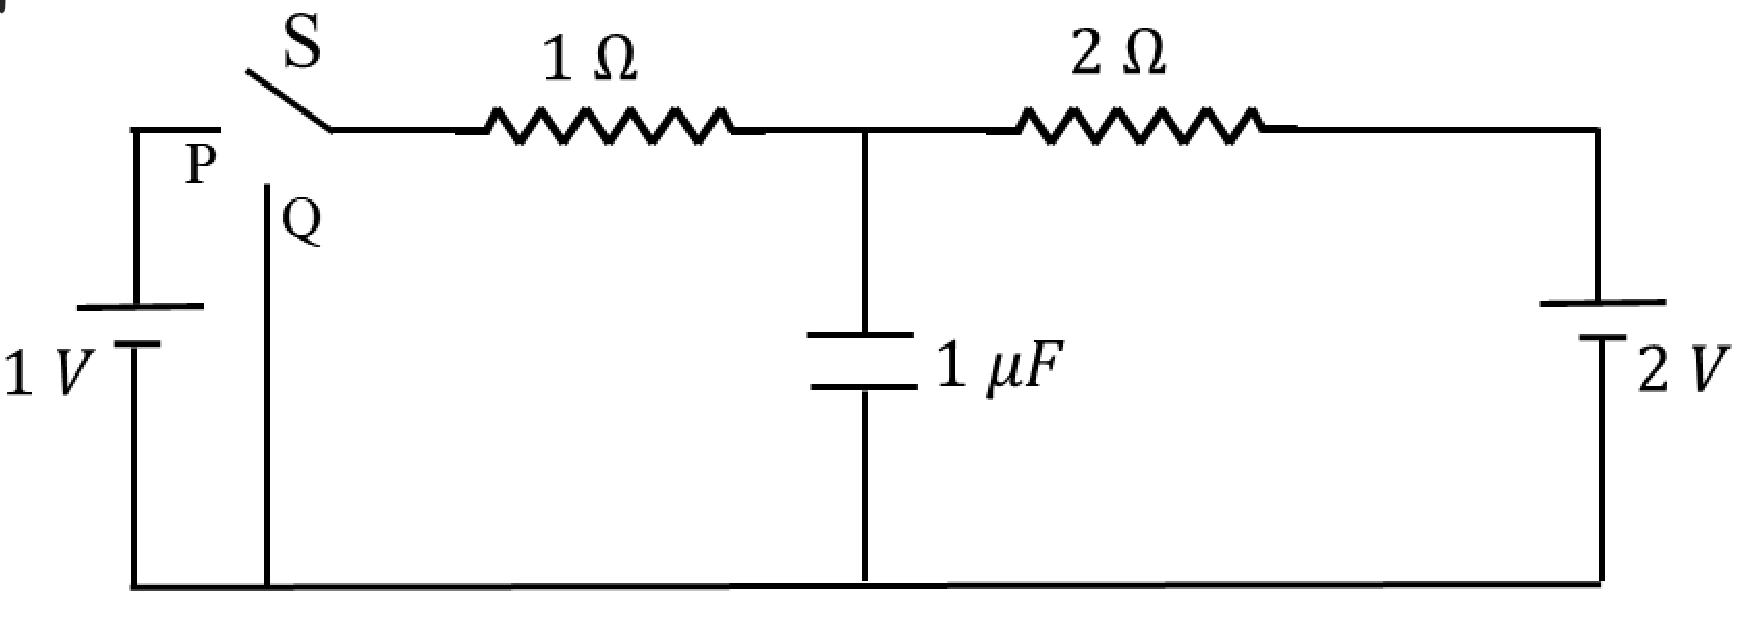
\includegraphics[width=\columnwidth]{Figs/ckt.jpg}
			\caption{}
			\label{fig:ckt}
\end{figure}
\item Draw the circuit using latex-tikz. \\
 \solution 
 \begin{figure}[!ht]
	  \begin{center}
	   \begin{circuitikz}
            \draw (0,0) 
             to [short] (8,0)
	     ;
	    \draw (8,3)
	     to [battery1,l_ = $2V$](8,0)
	     ;
	     \draw (0,3)
	     to [battery1,l_ = $1V$](0,0)
	     ;
	     \draw (8,3)
             to [R = $2\Omega$](4,3) 
	     to [R = $1\Omega$](1,3)
	     to [nos, l_ = S,mirror] (0,3) node[label = {left:P}]{}
	     ;
	     \draw (4,3)
	     to [C =  1 $\mu F$](4,0);
	     \draw (0.8,0)
	      to [short](0.8,2.7) node[label = {right:Q}]{}
	      
	      ;
	   \end{circuitikz}
   \end{center}
   \caption{Circuit diagram of the question}
   \label{circt-1}
\end{figure}
\item Find $q_1$.\\
 \solution Since the switch S is closed for a long time at P, the circuit at steady state looks like,
    \begin{figure}[!ht]
	 \begin{center}
	  \begin{circuitikz}
	  \draw (0,0) 
             to [short] (8,0)
	     ;
	    \draw (8,3)
	     to [battery1,i_ = $i$,l_ = $2V$](8,0)
	     ;
	     \draw (0,3)
	     to [battery1,l_ = $1V$](0,0)
	     ;
	     \draw (8,3)
             to [R = $2\Omega$](4,3) 
	     to [R = $1\Omega$](1,3)
	     to [short](0,3)
	     ;
	     \draw (4,3)
	     to [short,*-o](4,1.75)node[left]{$+$};
	     \draw (4,0)
	     to [short,*-o](4,1.25)node[left]{$-$};
	  \end{circuitikz}
	  \end{center}
     \end{figure}
	     Now if we apply KVL,
	 \begin{align}
		 2 - 2i-i -1 &=0 \\
	  \implies i &= \frac{1}{3}
	 \end{align}
	 The potential difference across capacitor is,
	  \begin{align}
		  V_{C} &= 2 - 2i \\
		        &= \frac{4}{3}
	  \end{align}
       Therefore the charge on capacitor will be,
        \begin{align}
	  q_{1} &= \frac{4}{3} \mu F
	 \end{align}
     \item Show that the Laplace transform of $u(t)$ is $\frac{1}{s}$ and find the ROC.\\
	     \solution From $\ref{eq:laplace}$ we can write laplace transform of unit step function $u(t)$ as,
	      \begin{align}
                 \mathcal{L}\cbrak{u(t)} &= \int_{-\infty}^{\infty}u(t)e^{-st}dt \\
					 &= \int_{0}^{\infty}e^-stdt \\
					 &=  \sbrak{\frac{e^{-st}}{-s}}_{0}^{\infty} 
	      \end{align}
	      For the laplace transform to exist,$Re\brak{s} >0$ using that
	       \begin{align}
		       \mathcal{L}\cbrak{u(t)} &= \frac{1}{s} \text{with ROC $Re\brak{s} >0$}
               \end{align}
	       The ROC plot looks like $\ref{Fig:ROC_1}$,
	 \begin{figure}[!ht]
	    \centering
	    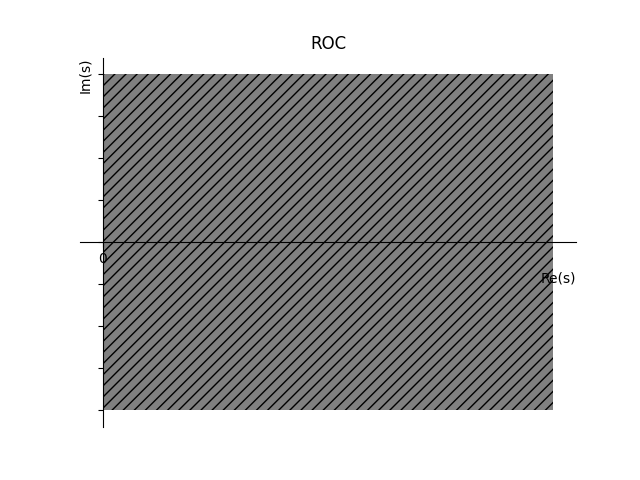
\includegraphics[width = \columnwidth]{Figs/2.4.png}
	    \caption {ROC of laplace transform of $u(t)$}
	    \label{Fig:ROC_1}
           \end{figure}
        \item Show that 
		\begin{align}
			e^{-at}u(t) \system{L} \frac{1}{s+a}, \quad a > 0
		\end{align}
		and find the ROC. \\
	 \solution The laplace transform will be,
	   \begin{align}
		   \mathcal{L}\cbrak{e^{-at}u(t)} &= \int_{-\infty}^{\infty}e^{-\brak{a+s}t}u(t)dt \\
						  &= \int_{0}^{\infty}e^{-\brak{a+s}t} dt \\
						  &= \sbrak{\frac{e^{-\brak{a+s}t}}{-\brak{a+s}}}_{0}^{\infty}
	   \end{align}
	   Now for the integral to exist,
	    \begin{align}
		    Re\brak{s+a} > 0 \\
		    Re\brak{s} > -a
	    \end{align}
	    So the ROC will be $Re\brak{s} > -a$ and with that ROC, 
	     \begin{align}
		     \mathcal{L}\cbrak{e^{-at}u(t)} &= \frac{1}{a+s}
	     \end{align}
	     And the ROC plot looks like $\ref{Fig:ROC_2}$,
	      \begin{figure}
	       \centering
	       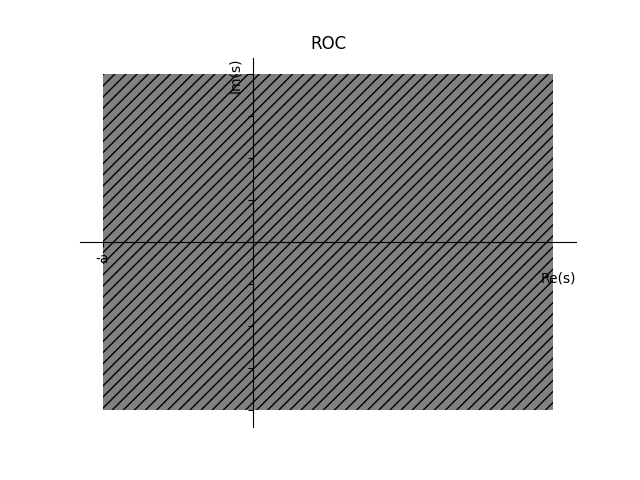
\includegraphics[width = \columnwidth]{Figs/2.5.png}
	       \caption{ROC of laplace transform of $e^{-at}u\brak{t}$}
	       \label{Fig:ROC_2}
	      \end{figure}
	\item Now consider the following resistive circuit transformed from 
			Fig. $\ref{fig:ckt}$
		\begin{figure}[!ht]
			\centering
			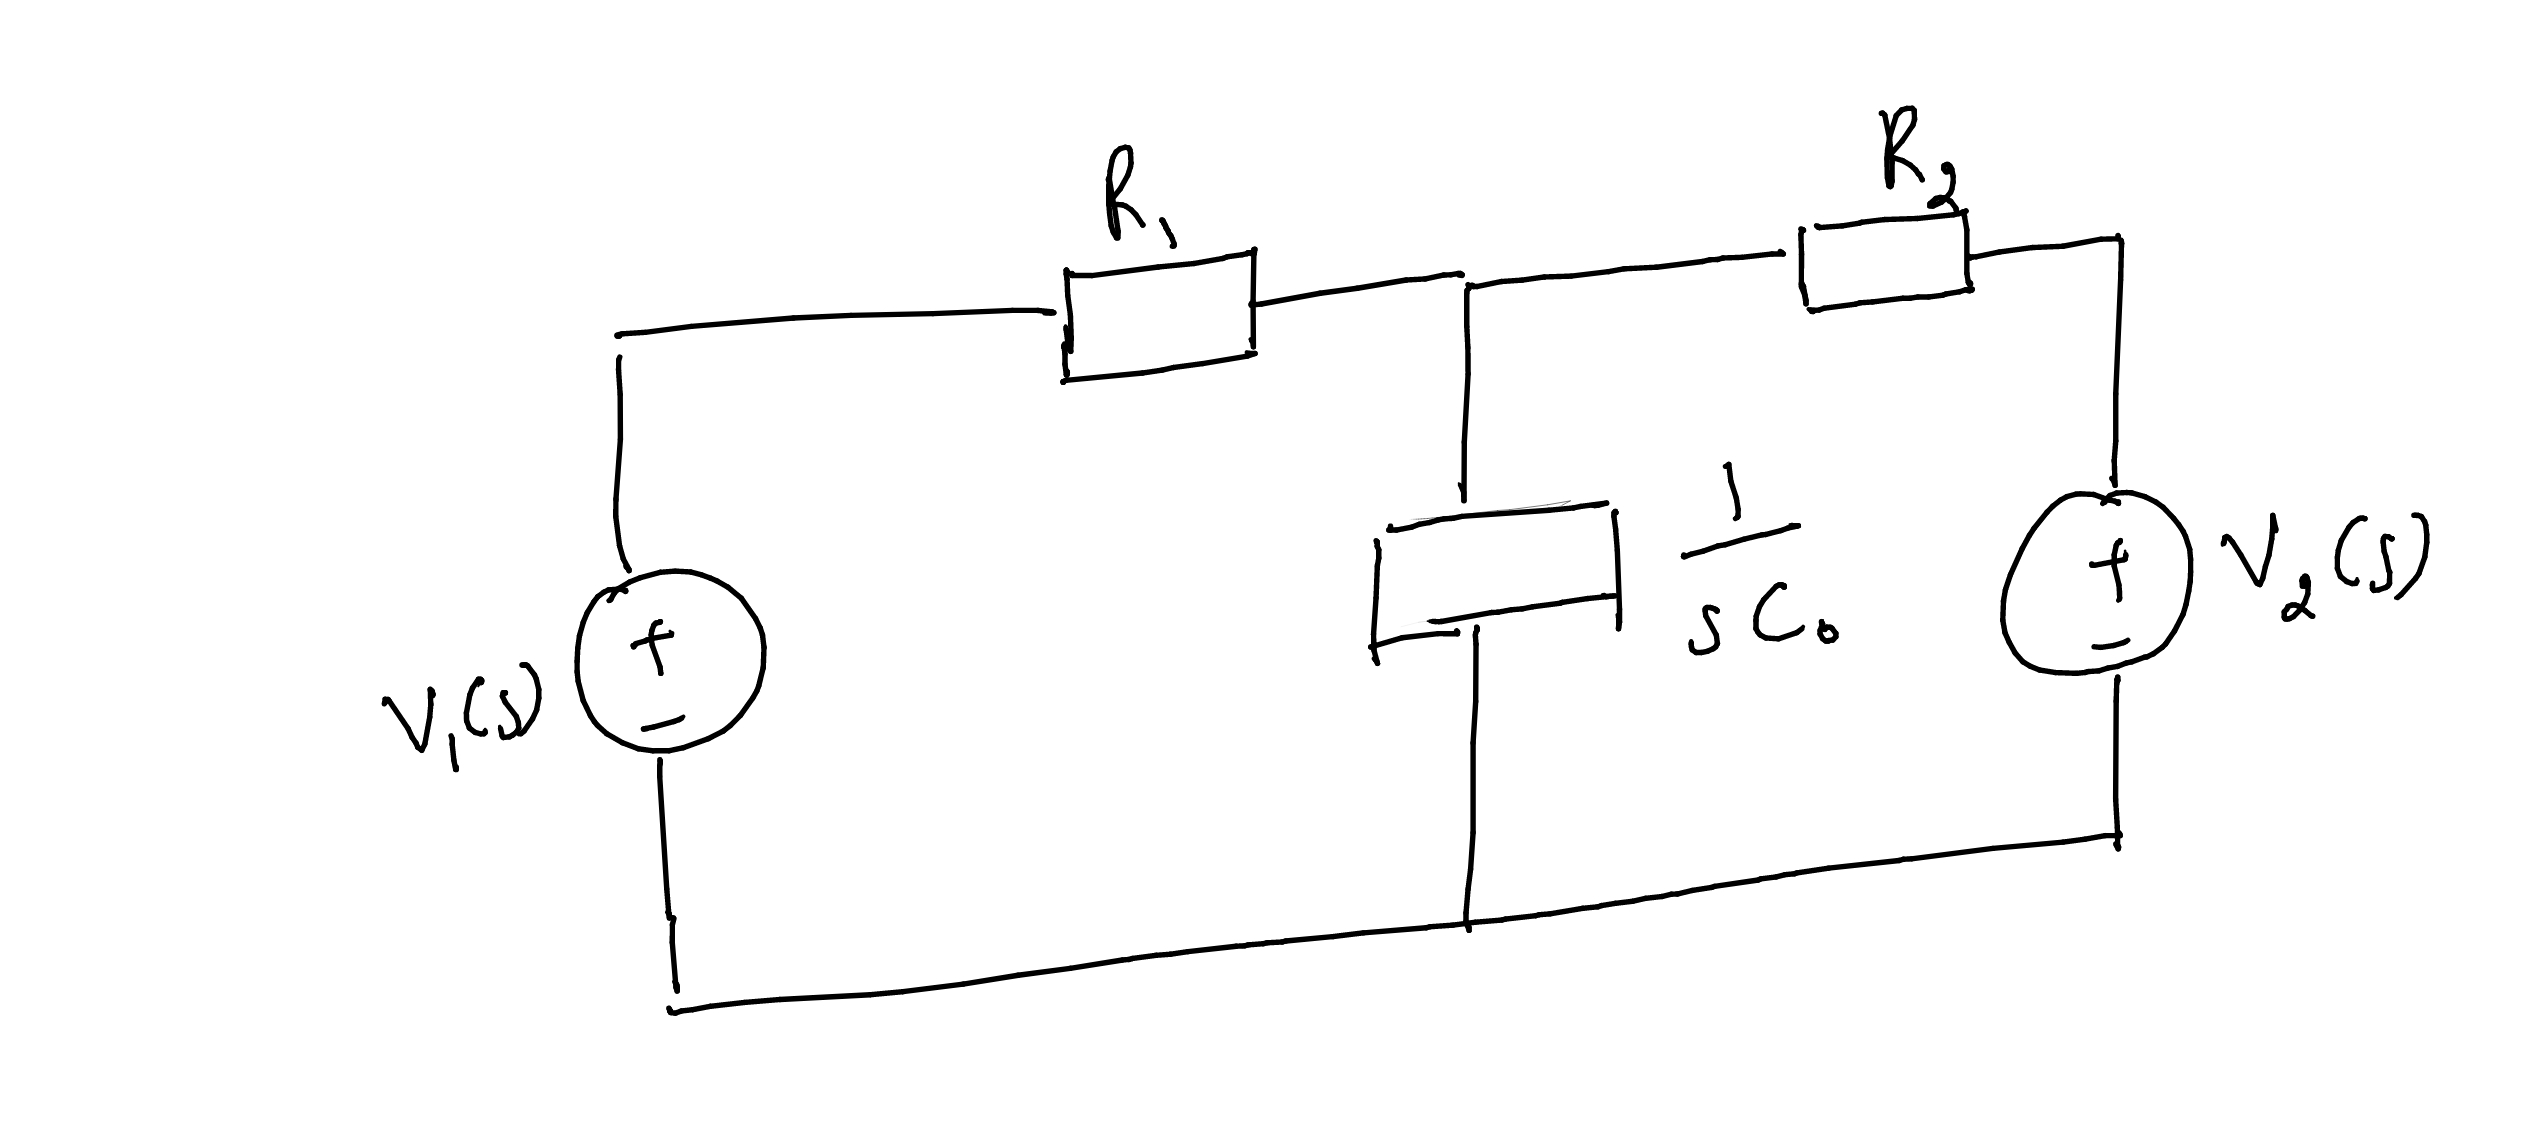
\includegraphics[width=\columnwidth]{Figs/lap-ckt.jpg}
			\caption{}
			\label{fig:lap-ckt}
\end{figure}
		where 
		\begin{align}
			u(t) \system{L} V_1(s)
			\\
			2u(t) \system{L} V_2(s)
		\end{align}
		Find the voltage across the capacitor $V_{C_0}(s)$.\\
	\solution From the earlier proved results,
	  \begin{align}
	    V_1(s) &= \mathcal{L}\brak{u(t)} \\
	           &= \frac{1}{s} \\
	    V_2(s) &= \mathcal{L}\brak{2u(t)} \\
		   &= \frac{2}{s}
	  \end{align}
	   Note that ROC here is $Re\cbrak{s} > 0$. \\
	  And the let the ends of resistive capacitor has voltages of $V_{C_0}$ and $0$. The same can be seen in figure $\ref{Fig-lap-ckt_2}$,
	  \begin{figure}[!ht] 
		\begin{center}
	         \begin{circuitikz}
			\draw (0,0)node[left]{$0$} 
			to [V,l_=$V_1(s)$](0,3)node[left]{$V_{1}$}
			to [generic ,l_ = $1 \Omega$](4,3)
			to [generic,l_ = $2 \Omega$](8,3)
                        ;
			\draw (8,0) node[below]{$0$}
			to [V,l_ = $V_2(s)$](8,3)node[above]{$V_2$}
                        ;
			\draw (4,3) node[above]{$V_{C_0}$}
			to [capacitor,l_ = $\frac{1}{sC_{0}}$](4,0) node[below]{$0$}
			;
			\draw (0,0)
			to [short] (8,0)
			;	
	        \end{circuitikz}
	       \end{center}
	       \caption{}
	       \label{Fig-lap-ckt_2}
          \end{figure} 
        If we apply Kirchoff's Junction law,
	 \begin{align}
		 \frac{V_{C_0} - V_1(s)}{1} + \frac{V_{C_0} - 0}{\frac{1}{sC_0}} \nonumber \\ + \frac{V_{C_0} - V_2(s)}{2}  &= 0 \\
		 V_{C_0}(s)\brak{\frac{3}{2} +sC_0} &= V_1(s) +  \frac{V_2(s)}{2} 
	 \end{align}
 Substituting $V_1(s), V_2(s)$ and $C_0$, you will get
          \begin{align}
		  V_{C_0}(s) &= \frac{4}{s\brak{3 +2x10^{-6}s}}\label{eq:lap-V_c}
	  \end{align}
	\item Find $v_{C_0}(t)$.  Plot using python.\\
	 \solution Now we can find the voltage of capacitor in time domain using inverse laplace transform,
	   \begin{align}
		   v_{C_0}(t) &= \mathcal{L}^{-1}\sbrak{\frac{4}{s\brak{3 +2x10^{-6}s}}} \\
			      &= \mathcal{L}^{-1}\sbrak{\frac{4}{3}\sbrak{\frac{1}{s} - \frac{1}{10^{-6}s + \frac{3}{2}}}} \\
			      &= \frac{4}{3}\mathcal{L}^{-1}\sbrak{\frac{1}{s}} - \frac{4}{3}\mathcal{L}^{-1}\sbrak{\frac{1}{s + \frac{3x10^6}{2}}} \\
			      &= \frac{4}{3}\brak{ u(t) - u(t)e^{-\frac{3x10^6t}{2}}} \\
		   \implies v_{C_0}(t) &= \frac{4}{3}\brak{1 - e^{-\frac{3t}{2}\text{x}10^6}}u(t)
	   \end{align}
	   Note that the ROC here is $Re\cbrak{s} > 0$.\\
	   The plot $\ref{Fig:V_c}$ of the same can be viewed using the python code in the following link,
	 \begin{lstlisting}
wget https://github.com/Charanyash/EE3900-Digital_Signal_Processing/tree/master/Circuits%20and%20Transforms/Codes/2.7.py
         \end{lstlisting}
Then run the following command,
      \begin{lstlisting}
python3 2.7.py
      \end{lstlisting}
      \begin{figure}[ht!]
	       \centering
	       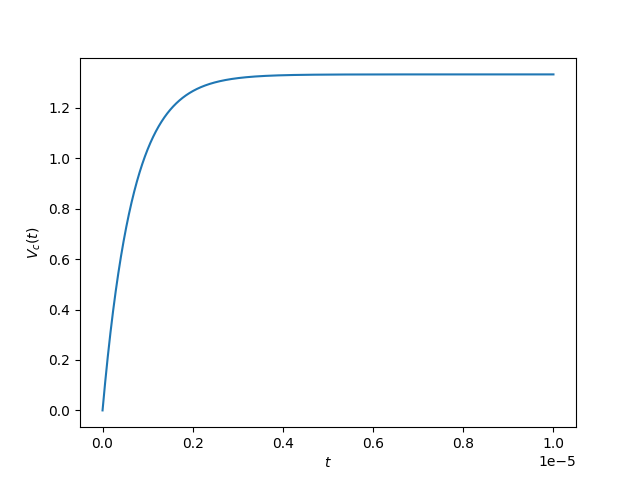
\includegraphics[width = \columnwidth]{Figs/2.7.png}
	       \caption{The plot of $V_c(t)$ vs $t$}
	       \label{Fig:V_c}
     \end{figure}	   
	\item Verify your result using ngspice.\\
	 \solution Download the codes from the below links, 
	   \begin{lstlisting}
wget  https://github.com/Charanyash/EE3900-Digital_Signal_Processing/tree/master/Circuits%20and%20Transforms/Codes/2.8.cir
wget https://github.com/Charanyash/EE3900-Digital_Signal_Processing/tree/master/Circuits%20and%20Transforms/Codes/2.8.py
           \end{lstlisting}
	   Then run the following command,
	\begin{lstlisting}
ngspice 2.8.cir
python3 2.8.py
	\end{lstlisting}
	\begin{figure}
	  \centering
	  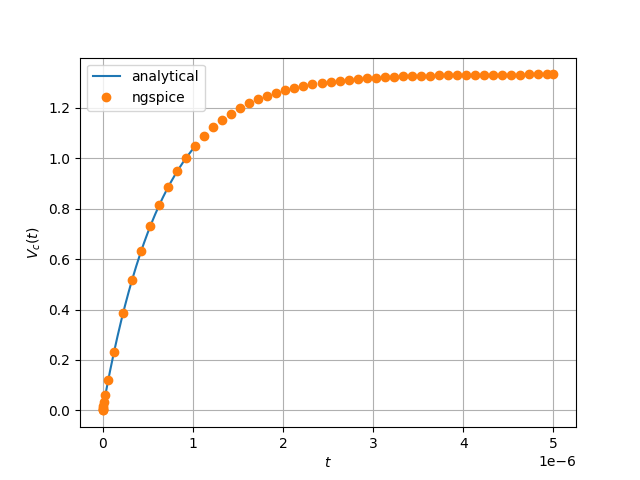
\includegraphics[width = \columnwidth]{Figs/2.8.png}
	  \caption{The plot of $V_c(t)$ vs $t$ using ngspice}
	  \label{Fig:V_c_ngspice}
	\end{figure}
       \item Obtain Fig. 
			$\ref{fig:lap-ckt}$
			using the equivalent differential equation.\\
	\solution Using Kirchoff's Junction Law in $\ref{fig:ckt}$,
	  \begin{align}
		  \frac{v_c(t) - v_1(t)}{1} + \frac{v_c(t) - v_2(t)}{2} + \frac{dq}{dt} &= 0 \label{eq:ckt_jun}
	  \end{align}
	  where $q(t)$ is the charge on capacitor. And can be written as ,
	   \begin{align}
		   q_c(t) &= Cv_c(t)  \label{eq:q_C}
	   \end{align}
	   Now applying laplace transform of $\eqref{eq:ckt_jun}$ using $\eqref{eq:q_C}$,
	   \begin{align}
		   \brak{V_c(s) - V_1(s)} + \frac{1}{2}\brak{V_c(s) - V_2(s)}  \nonumber \\ + C\brak{sV_c(s) - v_c(0^-)} &= 0
	   \end{align}
	   We know,
	    \begin{align}
	        v_c(0^-) = v_c(0) = 0
            \end{align}
            Using that,
	     \begin{align}
		 \frac{V_{C_0} - V_1(s)}{1} + \frac{V_{C_0} - 0}{\frac{1}{sC_0}} + \frac{V_{C_0} - V_2(s)}{2}  &= 0 
	     \end{align}
	     With this equation, we can write the equivalent resistive circuit as shown in Fig $\ref{fig:lap-ckt}$. 
\end{enumerate}
 \section{Initial Conditions}
\begin{enumerate}[label=\arabic*.,ref=\thesection.\theenumi]
\numberwithin{equation}{section}
\item Find $q_2$ in Fig. 
			$\ref{fig:ckt}$. \\
 \solution After closing switch at $Q$ for long time the circuit looks like $\ref{fig:q_2}$,
 \begin{figure}[!ht]
	  \begin{center}
	   \begin{circuitikz}
		   \draw (0,0) node[left]{$0$}
	      to [short](0,3)node[above]{$0$}
	      to [R,l_ = $1 \Omega$](4,3)node[above]{$V_c$}
	      to [R,l_ = $ 2 \Omega$](8,3)node[right]{$2$}
	      to [battery1 , l_= $2 V$](8,0) node[right]{$0$}
	      to [short] (0,0)
	      ;
	      \draw(4,3)
	      to [short,*-o](4,1.75) node[right]{$+$} 
	      ;
	      \draw(4,1.25)
	      to [short,*-o](4,0) node[right]{$-$}
	      ;	
            \end{circuitikz}
	   \end{center}
	   \caption{}
	   \label{fig:q_2}
\end{figure}
Now we will use Kirchoff's Junction Law in this circuit,
 \begin{align}
	 \frac{V_c -0}{1} + &\frac{V_c - 2}{2} = 0 \\
	 \implies V_c &= \frac{2}{3}V
 \end{align}
And the charge on the capacitor will be,
   \begin{align}
	 q_2 = \frac{2}{3} \mu C
   \end{align}
\item Draw the equivalent $s$-domain resistive circuit when S is switched to position Q.  Use variables $R_1, R_2, C_0$ for the passive elements.
Use latex-tikz.
		$\label{prob:init}$ \\
		\solution The equivalent $s$-domain resistive circuit looks like $\ref{fig:lap-ckt_q_2}$.
		\begin{figure}[!ht]
		\begin{center}
		\begin{circuitikz}
			\draw (0,0) 
			to [short] (0,3)node[left]{$0$}
			to [generic,l_=$R_1$] (4,3)
			to [generic,l_=$R_2$] (8,3)
			to [V,l_ = $V_2(s)$](8,0)
			;
			\draw (4,3) node[above]{$V_c(s)$}
			to [capacitor,l_ = $\frac{1}{sC_o}$](4,1.75)
			to [V, l_ = $\frac{4}{3s}$](4,0)
			;
			\draw(0,0)
			to [short](8,0)
			;
		\end{circuitikz}
		\end{center}
		\caption{Circuit after closing switch to Q in s-domain}
		\label{fig:lap-ckt_q_2}
		\end{figure}
		The battery $\frac{4}{3s}$ is added series to $C_0$ in s- domain by taking consideration of initial charge on capacitor $q_1 = \frac{4}{3} \mu C$ before closing switch to Q. 
	\item $V_{C_0}(s)$ = ?\\
		\solution Apply kirchoff's junction law in the s-domain circuit $\ref{fig:lap-ckt_q_2}$,taking $R_1 = 1 \Omega$ and $R_2 = 2 \Omega$
		    \begin{align}
			    \frac{V_{C_0}(s) - 0}{1} + \frac{V_{C_0}(s) - \frac{4}{3s}}{\frac{1}{sC_0}} &+ \frac{V_{C_0}(s) - V_2(s)}{2} = 0 \\
			    \implies V_{C_0}(s)\brak{\frac{3}{2} + sC_0} &= \frac{V_2(s)}{2} + \frac{4C_0}{3} \\
			    \implies V_{C_0}(s) &= \frac{\frac{1}{s} + \frac{4C_0}{3}}{\frac{3}{2} + sC_0} \\ 
		    \therefore V_{C_0}(s) = \frac{2\brak{3 + 4sC_0}}{3s\brak{3 + 2sC_0}}
		     \end{align}
	\item $v_{C_0}(t)$ = ? Plot using python.\\
	 \solution We can obtain the potential difference across the capacitor in time domain by applying inverse laplace transform under right ROC conditions,
	   \begin{align}
		   v_{C_0}(t) &= \mathcal{L}^{-1}\sbrak{\frac{2\brak{3 + 4sC_0}}{3s\brak{3 + 2sC_0}}} \\
			      &= \mathcal{L}^{-1}\sbrak{\frac{2}{3s} + \frac{4C_0}{3\brak{3 + 2sC_0}}} \\
			      &= \mathcal{L}^{-1}\sbrak{\frac{2}{3s}} + \mathcal{L}^{-1}\sbrak{\frac{4C_0}{3\brak{3 + 2sC_0}}}
           \end{align}
              With ROC condition $Re\cbrak{s} > 0$,
	       \begin{align}
		       v_{C_0}(t) &= \frac{2u(t)}{3} + \frac{2u(t)}{3}e^{-\frac{3}{2C_0}}
	       \end{align}
            Substituting $C_0 = 1 \mu F$,
	       \begin{align}
		       v_{C_0}(t) &= \frac{2}{3}\brak{1 + e^{-\frac{3x 10^6}{2}}}u(t)\label{eq:V_C_2}
	       \end{align}
             We can verify the same using the python code from the below link,
	      \begin{lstlisting} 
wget  https://github.com/Charanyash/EE3900-Digital_Signal_Processing/tree/master/Circuits%20and%20Transforms/Codes/3.4.py
	      \end{lstlisting}
	      Then run the following command,
	       \begin{lstlisting}
wget  python3 3.4.py
	       \end{lstlisting}
	       
		\begin{figure}[!ht]
			\centering
			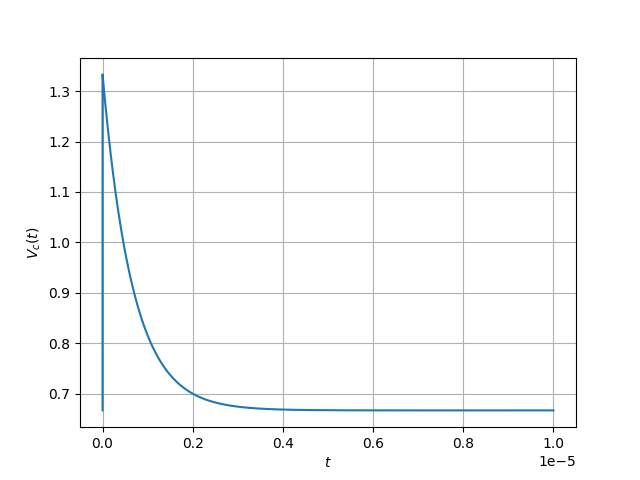
\includegraphics[width=\columnwidth]{Figs/3.4.png}
			\caption{The plot of $V_c(t)$ vs $t$}
			\label{fig:V_c_t_2}
\end{figure}
	\item Verify your result using ngspice. \\
	  \solution 
	     Download the codes from the below links
	      \begin{lstlisting}
wget  https://github.com/Charanyash/EE3900-Digital_Signal_Processing/tree/master/Circuits%20and%20Transforms/Codes/3.5.py	      
wget  https://github.com/Charanyash/EE3900-Digital_Signal_Processing/tree/master/Circuits%20and%20Transforms/Codes/3.5.cir
              \end{lstlisting}
    Then run the following commands,
     \begin{lstlisting}
ngspice 3.5.cir
python3 3.5.py
    \end{lstlisting}
		\begin{figure}[!ht]
			\centering
			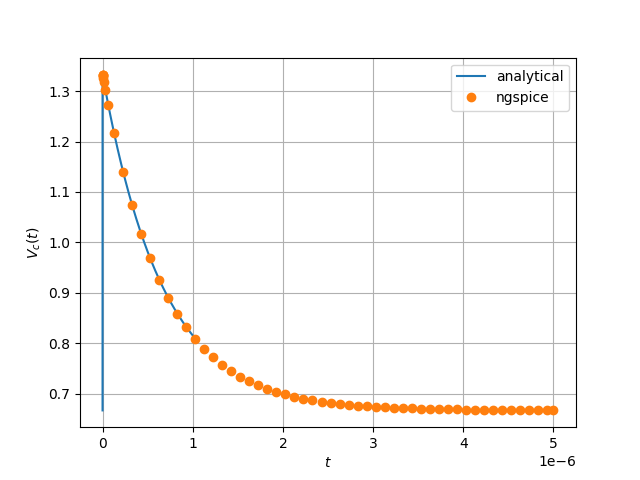
\includegraphics[width=\columnwidth]{Figs/3.5.png}
			\caption{The plot of $V_c(t)$ vs $t$ using ngspice}
			\label{fig:ngspice_2}
\end{figure}
\item Find $v_{C_0}(0-), v_{C_0}(0+)$ and  $v_{C_0}(\infty) $.\\
	\solution In that case when $t < 0$ switch is not closed to Q so the circuit will be in steady state $(\text{switch at P})$,
	  \begin{align}
		  v_{C_0}(0-) &= \sbrak{\frac{4}{3}\brak{1 - e^{-\frac{3x 10^6}{2}}}u(t)}_{t = \infty} \\
			      &= \frac{4}{3}V
	   \end{align}
	   And for $t = 0+$ and $t = \infty$, we can use $\eqref{eq:V_C_2}$,
	    \begin{align}
		    v_{C_0}(0+) &= \frac{4}{3}V \\
		    v_{C_0}(\infty) &= \frac{2}{3}V
	    \end{align}
\item Obtain the Fig.  in problem 
		$\ref{prob:init}$
			using the equivalent differential equation.\\
	\solution Using Kirchoff's Junction Law ,
	  \begin{align}
		  \frac{v_c(t) - v_1(t)}{1} + \frac{v_c(t) - v_2(t)}{2} + \frac{dq}{dt} &= 0
	  \end{align}
	  where $q(t)$ is the charge on capacitor. And can be written as ,
	   \begin{align}
		   q_c(t) &= Cv_c(t)  
	   \end{align}
	   Now applying laplace transform ,
	   \begin{align}
		   \brak{V_c(s) - V_1(s)} + \frac{1}{2}\brak{V_c(s) - V_2(s)}  \nonumber \\ + C\brak{sV_c(s) - v_c(0^-)} &= 0
	   \end{align}
	   We know,
	    \begin{align}
		    v_c(0^-) = \frac{4}{3}V
            \end{align}
            Using that,
	     \begin{align}
		     \frac{V_{C_0} - V_1(s)}{R_1} + \frac{V_{C_0} - \frac{4}{3s}}{\frac{1}{sC_0}} + \frac{V_{C_0} - V_2(s)}{R_2}  &= 0 
	     \end{align}
	     With this equation, we can write the equivalent resistive circuit as shown in Fig $\ref{fig:lap-ckt_q_2}$. 
 \end{enumerate}
\section{Bilinear Transform}
\begin{enumerate}[label=\arabic*.,ref=\thesection.\theenumi]
\numberwithin{equation}{section}
\item In Fig. 
			\ref{fig:ckt},
			consider the case when $S$ is switched to $Q$ right in the beginning. Formulate the differential equation.\\
			\solution When the switch $S$ is switched to $Q$ right from the beginning, the circuit looks like \ref{fig:ckt-Q} 
 \begin{figure}[!ht]
	  \begin{center}
	   \begin{circuitikz}
		   \draw (0,0) node[left]{$0$}
	      to [short](0,3)node[above]{$Q$}
	      to [R,l_ = $1 \Omega$](4,3)node[above]{$V_c$}
	      to [R,l_ = $ 2 \Omega$](8,3)node[above]{$V_2(t)$}
	      to [battery1 , l_= $2 V$](8,0) node[right]{$0$}
	      to [short] (0,0)
	      ;
	      \draw (4,3)
	       to [capacitor, l_ = $1 \mu F$](4,0)
	       ;
            \end{circuitikz}
	   \end{center}
	   \caption{}
	   \label{fig:ckt-Q}
\end{figure}
So similar what we did earlier we use Kirchoff's Junction Law, 
    \begin{align}
	    \frac{v_{c}(t) - 0}{1} +  \frac{dq}{dt} + \frac{v_c(t) - v_2(t)}{2} &= 0 \label{diff_eq}
    \end{align}
   where $q(t)$ is the charge on capacitor at time $t$ with initial conditions as,
    \begin{align}
	    q(0^-) = q(0) = 0
    \end{align}

 \item Find $H(s)$ considering the ouput voltage at the capacitor.\\
	 \solution Here $H(s)$ means transfer function, it relates the output $(\text{response})$ of the system to the given input. Here we are asked to consider voltage at the capacitor as the output. \\
	 For that first we will do laplace transform of the above differential equation $\eqref{diff_eq}$,
	  \begin{align}
		  \frac{V_c(s) -0}{1} + C\brak{sV\brak{s} - v_c(0^-)} + \frac{V_c(s) - V_2(s)}{2} &= 0
	  \end{align}
	  We know that  $v_c(0^-) = 0$ using that,
          \begin{align}
		  V_c(s)\brak{sC + \frac{3}{2}} &= \frac{V_2(s)}{2} \\
		  \frac{V_c(s)}{V_2(s)} &= \frac{1}{\brak{2sC + 3}}
	  \end{align}
         This will be the transfer function $H(s)$ and substituting $C = 1 \mu F$, you will get
	  \begin{align}
                H(s) &= \frac{5 \times 10^5}{s + 1.5 \times 10^6}
	  \end{align}
  \item Plot $H(s)$.  What kind of filter is it?\\
   \solution Download the python code from the below link for the plot,
           \begin{lstlisting} 
wget  https://github.com/Charanyash/EE3900-Digital_Signal_Processing/tree/master/Circuits%20and%20Transforms/Codes/4.3.py
	      \end{lstlisting}
	      Then run the following command
	 \begin{lstlisting}
wget python3 4.3.py
        \end{lstlisting}
	  \begin{figure}
	    \centering
	    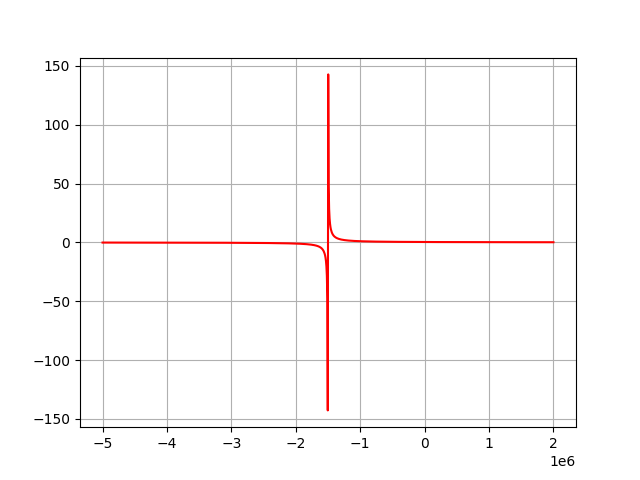
\includegraphics[width = \columnwidth]{Figs/4.3.png}
	    \caption{The plot of transfer function $H(s)$}
	    \label{fig:H(s)}
	  \end{figure}
Now if we consider frequency-domain transfer function by putting $s = j\omega$,
  \begin{align}
	  H(j\omega) &=\frac{5 \times 10^5}{j\omega + 1.5 \times 10^6} \\
	  \implies \abs{H(j\omega)} &=\frac{5 \times 10^5}{\sqrt{\omega^2 + \brak{1.5 \times 10^6}^2}}
  \end{align}
     As you can see , when $\omega$ increases the magnitude of transfer function $\abs{H(j\omega)}$ decreases.\\
     In other words, when the high frequency signals are passed as input their amplitudes will get diminished and filtered out. \\
     So this filter acts like a low-pass filter.
   \item Using trapezoidal rule for integration, formulate the difference equation
			by considering 
		\begin{align}
			y(n) = y(t)\vert_{t=n}
		\end{align}
		\solution To derive the difference equation, we will consider the differntial equation $\eqref{diff_eq}$,
    \begin{align}
	    \frac{v_{c}(t) - 0}{1} +  \frac{dq}{dt} + \frac{v_c(t) - v_2(t)}{2} &= 0 \\
	    \frac{v_{c}(t) -0}{1} + C\frac{dv_{c}(t)}{dt} + \frac{v_c(t) - v_2(t)}{2} &= 0
    \end{align}
    \begin{align}
	    C\frac{dv_{c}(t)}{dt} &= \frac{v_2(t) - 3v_c(t)}{2}\\
	    \implies v_{c}(t)\vert_{t = n}^{n+1} &= \frac{1}{C}\int_{n}^{n+1}\frac{v_2(t) - 3v_c(t)}{2} dt
    \end{align}
    Here we can use trapezoidal rule of integration for $n = 1 (\text{no.of sub intervals})$,
     \begin{align}
	     \int_{a}^{b}f(x)dx \approx \frac{b-a}{2}\brak{f(a) + f(b)}
     \end{align}
     Along with this rule,considering that $y(t) = v_c(t)$ and $y(n) = y(t)\vert_{t=n}$ we can write that
      \begin{align}
           y(n+1) - y(n) &= \frac{1}{2C}\brak{\frac{v_2(n) + v_2(n+1)}{2}} \nonumber \\
                    &- \frac{1}{2C}\frac{3\brak{y(n) + y(n+1)}}{2}
      \end{align}
      Now using the fact that $v_2(t) = 2u(t)$,
       \begin{align}
        y(n+1) - y(n) &= \frac{1}{2C}\brak{u(n) + u(n+1)} \nonumber \\ & -\frac{1}{2C}\frac{3\brak{y(n) + y(n+1)}}{2} \\
	\implies y(n+1)\brak{1 + \frac{3}{4C}} &= y(n)\brak{1  - \frac{3}{4C}} \\ \nonumber &+ \frac{u(n) + u(n+1)}{2C}\label{eq:y_diff}
       \end{align}
       This will be the difference equation.
	\item Find $H(z)$.\\
	 For that we will find the z transform of $y(n)$ by applying z-transform on the difference equation,
	  \begin{align}
		  zY(z)\brak{1 + \frac{3}{4C}} &= Y(z)\brak{1 - \frac{3}{4C}} + \frac{1}{2C}\brak{\frac{1 + z}{1 - z^{-1}}}\\
		 \implies Y(z) &= \frac{\frac{1}{2C}\brak{\frac{1 + z}{1 - z^{-1}}}}{\frac{3}{4C}\brak{z+1} + z-1}
	  \end{align}
	  Now assume that
	    \begin{align}
		    x(n) &= x(t)\vert_{t=n}
	    \end{align}
	    And here, 
	    \begin{align}
	    x(t) = v_2(t) = 2u(t)\brak(\because v_2(t) = 2V \forall t \geq 0)\\
	    \implies x(n) = 2u(n)
	    \end{align}
	     So the z-transform of $x(n)$ will be,
	      \begin{align}
		X(z) &= \frac{2}{1 - z^{-1}}
	      \end{align}
	      with ROC being
	       \begin{align}
		       \abs{z} > 1
		\end{align}
	 Now our function of interest,transfer function in z-domain $H(z)$ will be
	  \begin{align}
		  H(z) &= \frac{Y(z)}{X(z)} \\
		       &= \frac{\frac{1}{2C}\brak{1 +z}}{\frac{3}{2C}\brak{z + 1} + 2\brak{z - 1}} 
	  \end{align}
            Using that $C = 1 \mu F$,
	     \begin{align}
		     H(z) &= \frac{\brak{1 + z^{-1}}2.5 \times 10^5}{z^{-1}\brak{7.5 \times 10^5 - 1} + 7.5\times 10^5 + 1}
	     \end{align}
	     with ROC being
	      \begin{align}
		      \abs{z} > max\cbrak{1,\abs{\frac{7.5 \times 10^5 - 1}{7.5 \times 10^5 + 1}}}\\
		\implies \abs{z} > 1
	      \end{align}
	\item How can you obtain $H(z)$ from $H(s)$?\\
		\solution The Bilinear Transform is a first-order approximation of natural logarithm function that is an exact mapping between z-plane to the s-plane.\\
		Here to get z-transform of a discrete-time sequence from its corresponding laplace transform, where each element is attached with corresponding unit impulse, we will approximate the below fact,
		 \begin{align}
			 s = \frac{\ln\brak{z}}{T}
		 \end{align}
		 where $T$ is the step size.\\
		 If we expand the natural logarithm,
		  \begin{align}
			  s = \frac{2}{T}\sbrak{\brak{\frac{z-1}{z+1}} + \frac{1}{3}\brak{\frac{z-1}{z+1}}^3 + \cdots}\\
			  s \approx \frac{2}{T}\frac{z -1}{z + 1} \\
			  s \approx \frac{2}{T}\frac{1 - z^{-1}}{1 + z^{-1}}
		  \end{align}
	Here $T = 1$ .So,
	 \begin{align}
		 H(s)\vert_{s = 2\frac{1 - z^{-1}}{1 + z^{-1}}} &= \frac{5 \times 10^5}{2\frac{1 - z^{-1}}{1 + z^{-1}} + 1.5 \times 10^6} \\
								&= \frac{2.5 \times 10^5\brak{1 + z^{-1}}}{\brak{1-z^{-1}} + 7.5 \times 10^5\brak{1 + z^{-1}}} \\
								&= \frac{\brak{1 + z^{-1}}2.5 \times 10^5}{z^{-1}\brak{7.5 \times 10^5 - 1} + 7.5\times 10^5 + 1} \\
								&= H(z)
	 \end{align}
        \item Find $y(n)$ from $H(z)$ and verify whether $y(n) = y(t)\vert_{t = n}$.\\
	 \solution 
	 \begin{align}
		 &Y(z) = H(z)X(z) \\
		      &= \frac{2.5 \times 10^5\brak{1 + z^{-1}}}{z^{-1}\brak{7.5 \times10^5 -1} + 7.5\times 10^5 + 1}\frac{2}{1 - z^{-1}} \\
		      &= \frac{2}{3}\sbrak{\frac{1}{1-z^{-1}} - \frac{2}{3} \frac{1}{\brak{7.5 \times 10^5 - 1}z^{-1} + \brak{7.5 \times 10^5 +1}}}
	 \end{align}
	 Now if we apply inverse z-transform by taking ROC $\abs{z} > 1$,
	  \begin{align}
		  y(n) &= \frac{2}{3}u(n) - \frac{2}{3}\brak{-\frac{7.5 \times 10^5 -1}{7.5 \times 10^5 + 1}}^nu(n)
	  \end{align}
	  Here we used the following properties of z-transform,
	   \begin{align}
		   u(n) \ztrans \frac{1}{1-z^{-1}} , \abs{z} > 1\\
		   a^{n}u(n) \ztrans \frac{1}{1 - az^{-1}} ,\abs{z} >\abs{a}
	   \end{align}
	   Here we are sampling the signal at high frequency means at small intervals of time let say for $n = 0.5 \times 10^{-5} , 1 \times 10^{-5} \cdots$,for that we can approximate $y(n)$ as,
	    \begin{align}
		    y(n) \approx \frac{2}{3}\brak{ 1 - \frac{1 - 7.5 \times 10^5n}{1 + 7.5\times 10^5n}}u(n)
	    \end{align}
            Now we will verify it from $y(t)$, for that consider
	     \begin{align}
		     Y(s) &= H(s)X(s) \\
			  &=\frac{5 \times 10^5}{s + 1.5 \times 10^6}\frac{2}{s} \\
			  &= \frac{2}{3}\brak{\frac{1}{s} - \frac{1}{s + 1.5 \times 10^6}}
	     \end{align}
	     Now we will apply inverse laplace transform with ROC being $\mathcal{R}\cbrak{s} > 0$ on b.s,
	      \begin{align}
	           y(t) &= \frac{2}{3}\brak{1 - e^{-1.5\times 10^6t}}u(t)
              \end{align}
               Now 
	        \begin{align}
			e^{-1.5 \times 10^6t} &= \frac{e^{-7.5 \times 10^5t}}{e^{7.5 \times 10^5t}} \\
			&\approx \frac{1 - 7.5\times10^5t}{1 + 7.5\times10^5t} , \text{when}\, t << 10^{-6}
		\end{align}
	Using that,
	     \begin{align}
		     y(t) &= \frac{2}{3}\brak{1 - \frac{1 - 7.5\times10^5t}{1 + 7.5\times10^5t}}u(t)
	     \end{align}
	     And 
	      \begin{align}
		      y(t)\vert_{t = n} &= \frac{2}{3}\brak{1 - \frac{1 - 7.5\times10^5n}{1 + 7.5\times10^5n}}u(n)
              \end{align}
          As you can see both are turn to be the same.\\
	  Download the following codes for the simulation and plot \ref{fig:y_n} 
	   \begin{lstlisting}
wget  https://github.com/Charanyash/EE3900-Digital_Signal_Processing/tree/master/Circuits%20and%20Transforms/Codes/4.7.cir
wget  https://github.com/Charanyash/EE3900-Digital_Signal_Processing/tree/master/Circuits%20and%20Transforms/Codes/4.7.py
           \end{lstlisting}
	   Then run the following command,
	\begin{lstlisting}
ngspice 4.7.cir
python3 4.7.py
        \end{lstlisting}
        \begin{figure}[!ht]
		\centering
		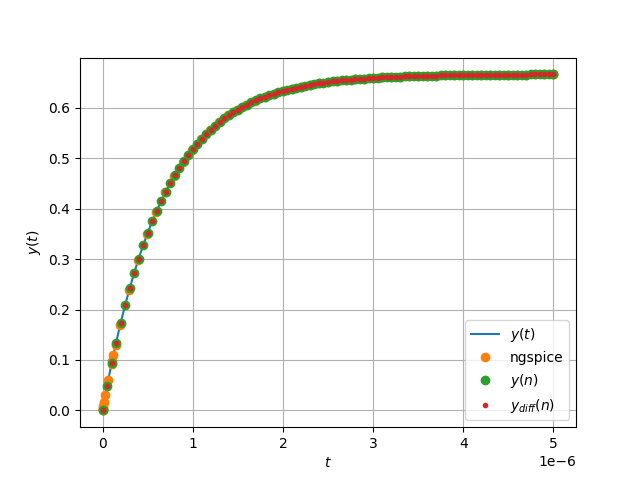
\includegraphics[width = \columnwidth]{Figs/4.7.png}
		\caption{Output of the filter vs time}
		\label{fig:y_n}
        \end{figure}
      \item Derive the expression for $y(n)$ using difference equation.\\
	      \solution Consider the difference equation $\eqref{eq:y_diff}$,
	       \begin{align}
		 y(n+1)\brak{1 + \frac{3}{4C}} &= y(n)\brak{1  - \frac{3}{4C}} \\ \nonumber &+ \frac{u(n) + u(n+1)}{2C} \\
		\implies y(n+1) &= y(n)\brak{\frac{1 - \frac{3}{4C}}{1 + \frac{3}{4C}}} + \frac{u(n) + u(n+1)}{2C + \frac{3}{2}}
	       \end{align}
	       Since our discussion is in $n > 0$, we can write
	        \begin{align}
			u(n) + u(n+1) & =2
		\end{align}
                Now let say a,b are coefficients in difference equation,
		 \begin{align}
			 a &= \frac{1 - \frac{3}{4C}}{1 + \frac{3}{4C}} \\
			   &= \frac{1 - 7.5\times 10^5}{1 + 7.5\times 10^5}\\
			 b &= \frac{2}{2C + \frac{3}{2}} \\
			   &= \frac{10^6}{1 + 7.5\times 10^5}
		 \end{align}
		So our difference equation looks like,
		 \begin{align}
			 y(n+1) &= ay(n) + b \\
			 y(n)   &= ay(n-1) + b\\
			        &= a\brak{ay(n-2) + b} + b \\
				&= a^2y(n-2) +ab + b \\
				& .. \nonumber \\
				& = a^ny(0) + b\brak{1 + a + \cdots +a^{n-1}}
		 \end{align}
		We know that $y(0) = 0$,
		 \begin{align}
			y(n) &= b\frac{1 - a^n}{1 - a}
		 \end{align}
		 And substituting the values of $a$ and $b$,
		  \begin{align}
			  y(n) &= \frac{10^6}{1 + 7.5\times 10^5} \frac{1 - \brak{\frac{1 - 7.5 \times10^5}{1 + 7.5 \times 10^5}}^n}{1 - \brak{\frac{1 - 7.5\times 10^5}{1 + 7.5 \times 10^5}}} \\
			       &= \frac{10^6}{1 + 7.5\times 10^5} \frac{1 - \brak{\frac{1 - 7.5 \times10^5}{1 + 7.5 \times 10^5}}^n}{\frac{1.5 \times10^6}{1 + 7.5\times 10^5}}\\
			       &= \frac{2}{3}\brak{1 - \brak{\frac{1 - 7.5 \times10^5}{1 + 7.5 \times 10^5}}^n}
		  \end{align}
		  And for $n << 10^{-6}$,
		    \begin{align}
			    y(n) \approx \frac{2}{3}\brak{1 - \frac{1 - 7.5 \times 10^5n}{1 + 7.5 \times10^5n}}
		    \end{align}
		    In general,we can write
		     \begin{align}
			     y(n) &= \frac{2}{3}\brak{1 - \frac{1 - 7.5\times 10^5n}{1 + 7.5 \times 10^5n}}
		     \end{align}
		As you can see it is similar to what we got earlier.
	\end{enumerate}
\end{document}
